\chapter{Sensitivity Analysis} \label{ch:sa}

% - why deterministic
%     --> what is stochastic and why we can treat it as deterministic:
%         - stochasticity in the population synthesis
%         - stochasticity in the boarding priority (negligible)

% - borgonovo protocol
%         - outputs
%         - goal
%         - elements
%         - methods
%         - values
%         - visualization
        
% - visualizations & results & comments vari 


%%%%%%%%%%%%%%%%%%%%%%%%%%%%%%%%%%%%%%%%%%%%%%%%%%%%%%%%%%%%%%%%%%%%%%%%%%%%%%%%%%%%%%%

\section{Preliminaries} \label{sec:ch4_pre}

The first thing to understand in order to set up the sensitivity analysis of an agent-based model is whether the model under study is stochastic or deterministic. Let us recall the difference between the two frameworks: a model is \textit{deterministic}, if by fixing its input, the output remains unchanged when evaluating the model multiple times; alternatively, a model is \textit{stochastic} if it produces a random value any time it is run with the same fixed input. The nature of the model dictates the kind of output one is going to investigate and the course of the analysis to perform. In the case of a stochastic model, one would want to compute descriptive statistics of the conditional distribution of the output given the fixed values of the inputs, and this requires to evaluate a sufficient number of samples, in order to average out the random component in the output, making the analysis more computationally expensive. If the model is deterministic, instead, one simulation run per each value of the inputs is enough to be able to assess the uncertainty in the outputs. \\ So, before diving deep into the analysis, let us briefly recap the model under study in this research, which has been explained in detail in Chapter \ref{ch:model}, to understand its nature and plan the next steps of the analysis accordingly. The idea of the model is to reproduce the flow of passengers using Milan's transportation network, in order to evaluate the efficiency of the system.
\begin{figure}
    \centering
    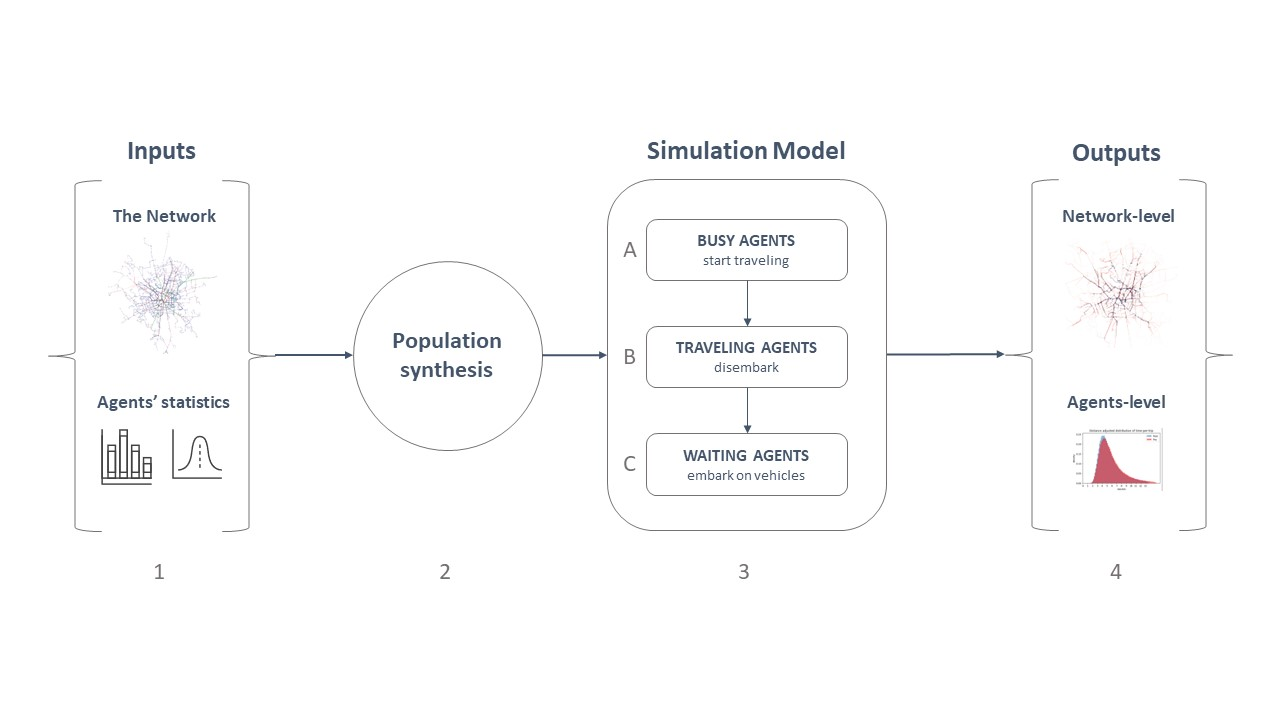
\includegraphics[width = \textwidth]{tex/pics/model_ppt2.jpg}
    \caption{Diagram representing the sequence of steps characterizing the agent-based model under study in this research.}
    \label{fig:model_schema}
\end{figure}
Figure \ref{fig:model_schema} portrays the main phases of the model. On the left side, there are the inputs that need to be fed to the simulator, which can be divided into those needed to construct the network, that will be the environment of the ABM, and those related to the distribution of agents' characteristics. Once one has collected all the inputs, the first step is to run the synthesis of the population. The goal of this phase is to obtain a fictitious population of agents which is as similar as possible to Milan's population, with respect to age, geographical residence and activities performed during an ordinary weekday. Next, the agents obtained are fed, together with the network, to the simulator: as soon as the simulation starts, they begin to move on the network to reach the location of the activities they have to perform. At the end of the simulation, the researcher is able to collect outputs related to the network (e.g. the most overloaded lines) or to the agents (e.g. traveling and waiting time), both at the individual and collective level. 
We can easily recognize two sources of stochasticity in the model's structure:
\begin{itemize}
	\item \textbf{the population synthesis} (2);
	\item \textbf{the boarding priority for waiting passengers} (C). 
\end{itemize}
I will now go through each of the two, in order to show that the impact of their stochastic nature on the model's results is negligible. In other words, for the purpose of the sensitivity analysis, from now on we will treat the model as if it were deterministic, that is, as if we obtain the same identical results from each model run, once the network, the population distributions and the number of agents has been fixed. This would allow us to perform one single run for each parameter setting and make the analysis less computationally expensive.

\paragraph{The population synthesis} 
As described in Section \ref{sec:3.3}, in order to construct the profile of each agent, features like age class, geographical residence and kind of activities performed are drawn from their respective distributions, which have been extrapolated from real demographic data about the residents of Milan. The population synthesis is, thus, a stochastic procedure, producing, at each run, a possibly different sample of agents. The problem with this stochasticity is that agents behavior in the simulations depend on their characteristics. In paricular, the probability of living in a specific zone of the city and that of performing a certain activity are conditional on the age class the agent belongs to, and how busy are agents is among the main drivers of traffic on the network. Moreover, agents' destinations depend on the activity they have to perform, which, again, depends on the age class. In an agent-based model, the results are determined by the collective behavior of agents. Hence, running the simulations with any specific set of individuals would lead to unique results and possibly to the emergence of a distinct phenomenon. For example, in our model, if the number of agents in a sample having the same destination is above average, then the results of the simulation would be biased, as they could show a particular overload on lines that lead to that specific destination. Since one wishes to eliminate, from the bias in the results, the component which depends on the population synthesis, a best practice would be to evaluate the model with multiple batches of agents and then agerage results across simulations. However, one can demonstrate that a large sample size ensures to achieve enough stability in the proportions of the agents' characteristics, across different samples resulting from the population synthesis procedure. That is, if the sample size is large enough, then the empirical distribution of agents will resemble the true distribution and one can decide to treat each sample as if they were equivalent, producing similar results. This kind of analysis can be included in the process of validating the population synthesis, as to assess its robustness. Indeed, in Section \ref{ssec:3.3.1}, I compared 100 samples of synthetic agents, of which I observed the distributions of multiple characteristics. Results show that, with a sample size of 20000, variability across samples is low. Hence, I decide to set default sample size to 20000 and disregard the stochasticity in the agents' profiles creation for the purposes of the sensitivity analysis.

\paragraph{Waiting agents' boarding priority}
As explained in \ref{sec:3.4}, at each timestep, agents are moved one at a time, and waiting agents are the last to move, as they are allowed to embark on the vehicle only after traveling agents disembark. While agents having to disembark are always allowed to do so (since there is no capacity associated to stops), those who have to get on a vehicle may be stopped by the constraint that such vehicle has already reached full capacity and forced to wait for the next available mean. Hence, for waiting agents, the boarding order is important. Indeed, and allowing always the same agent to be the first to get on a vehicle would drastically reduce someone's waiting time and increase someone else's.
In principle, for the purpose of this analysis I am only interested in the collective behavior of agents, and I am not going to inspect agents' individual behavior, as to follow the main scope of the model, that is, evaluating the public transportation system as a whole. So, any boarding priority strategy would be equally valid. However, to be more realistic, I assign the priority with which waiting agents embark on their preferred vehicle at random. More formally, given $c$ the remaining capacity of the vehicle and $w$ the number of waiting agents, we treat each $j$ of the $w$ agents as if they had the same probability of being the $i$-th to embark, for $i = 1, ..., c$, that is, $P[O_j = i] = \frac{1}{c}$, where $O_j$ is the random variable representing the order of embarking for agent $j$. Intuitively, given a list of waiting agents, at each timestep the list is randomly shuffled, and the first in the list gets to be the first to move. This is not the only possible strategy. Indeed, one could think of moving agents according to some fixed index, but, as a consequence, the ones with the lowest indices would always be the first to embark and to disembark, exhibiting unrealistically low waiting times, while the opposite would happen for the last agents evaluated. Alternatively, another possibility could be to follow a decreasing order in waiting time, letting the agents arrived earlier at each stop moving first. However, this strategy requires making more computations at each timestep, while the adopted strategy seems a reasonable compromise which allows being realistic and avoids giving the first-mover advantage always to the same agents. The problem is that, being this a stochastic strategy, it may happen that running twice the simulation with the same sample of agents would lead to different individual results, meaning the same agent could be waiting more or less across different simulations with identical inputs. Since I am only going to evaluate aggregate results (e.g. mean traveling time, mean waiting time, ...) and neglect individual patterns, I can safely ignore the stochasticity in boarding priority and treat this step as deterministic. Being the boarding procedure the only source of stochasticity in the simulation model, we can conclude that there is no source of significant stochasticity and assume the model has deterministic nature.

%%%%%%%%%%%%%%%%%%%%%%%%%%%%%%%%%%%%%%%%%%%%%%%%%%%%%%%%%%%%%%%%%%%%%%%%%%%%%%%%%%%%%%%

\section{Sensitivity analysis steps} \label{sec:ch4_steps}

\paragraph{Output of interest}
The first step of the sensitivity analysis design consists in choosing the output or outputs of interest. Having determined that the model under study in this research can be treated as deterministic, its outputs are going to be numerical quantities rather than distributions. Among the possible outputs of interest resulting from the simulations, I focus my analysis on three of them, which I believe reflect different characteristics of the system:
\begin{itemize}
    \item \textbf{The mean waiting-time-per-destination across agents.} Waiting time is an indicator of passengers' dissatisfaction: agents waiting less are happier about the system. Thus, although this is clearly an agent-related metric, one can think of it also as an index of network's efficiency. One would expect that this quantity is affected by changes in the values of different parameters characterizing the network, for example vehicles' speeds: if a vehicle is percieved as faster then more agents would like to use it, causing overload and, as a consequence, higher mean waiting time.
    \item \textbf{The mean and median traveling-time-per-km across trips.} During the simulation, I collect the time it takes agents to reach each destination in their schedule and the length in km of the path they traverse. The ratio between these two quantities, aggregated across trips, constitutes an output decision-makers could be interested in. Indeed, unlike waiting time, which only depends on lines' timetables and on whether vehicles are full or not, traveling time clearly depends on the distance to travel. Instead, traveling-time-per-km is a measure of agents' satisfaction, and, as a consequence, an index of network's efficiency.
    \item \textbf{The mean and median time edges reach full capacity.} This is a proxy for network overload, thus a direct measure of the system's efficiency. Indeed, one would like edges, and, in turn, vehicles, to have enough capacity to satisfy passengers' demand. The higher is, on average, this metric, the more overloaded are vehicles, and the less efficient is the network. I expect this quantity to be affected by changes in the network properties: in particular, adding more edges to the network, that is, adding transportation lines or connections among the existing lines, one would expect a lower network overload.
\end{itemize}
During the simulations I colect additional interesting quantities, such as the percentage of "finished" agents or the average number of vehicles used by agents in a day. In particular, the first should be close to 1 in a perfectly working system, but that is not always the case in our simulations and one would want to inspect which parameters influence variations in its values. Instead, the average number of vehicles is another indicator of agents' satisfaction, as typically passengers prefer to minimize the number of changes in their path, in order to have a smoother experience. For reasons of space, I decided not to focus on these metrics in my research, but they could be used to perform further analysis in the future.


\paragraph{Goal}
This sensitivity analysis has two main goals:
\begin{enumerate}
    \item \textbf{Factor prioritization and factor fixing}, that is, identifying the main driver of the output variations, for which a more accurate calibration is needed, and the least influential parameters, which one would like to fix to reduce complexity of the model;
    \item \textbf{Direction of change}, meaning I am interested in the sign of the outputs' variations due to changes of input values, to gather managerial insights;
    \item \textbf{Interaction quantification}, to recognize the effects of variations of the values of multiple parameters at the same time. 
\end{enumerate}


\paragraph{Elements}
% {'foot_r', 'speeds', 'am_counts_df', 'p_long', 'agents_strategy'}
In Section \ref{sec:3.4}, I described the model in terms of the structure proposed by \textcite{Borgonovo2022SensitivityAO}, and, in paricular, I highlighted the most relevant parameters and procedures. Among the elements presented, I will vary 3 environment-related parameters, 1 agents-related parameter and 1 procedure:
\begin{itemize}
    \item $\mathbf{r_{foot}}$, the maximum distance (in meters) used to consider two stops as "at walking distance". Setting a higher value for this parameter corresponds to possibly adding more edges to the graph representing the transportation network, making it denser.
    \item \textbf{vehicles' speeds vector}, a vector containing the commercial speeds (average speed over stretches) of the different kinds of transportation means. What truly influences the choice of a specific mean of transport is not the absolute value of its speed, but the relative magnitude with respect to the other means' speeds. Changing the relative sizes, agents' paths may be modified, in favor of more convenient solutions, and that could have an impact on traveling times and agents' experience in general.
    \item $\mathbf{r_{pois}}$, the maximum distance (in meters) used to consider a point of interest as "close" to a stop. 
    \item $\mathbf{p_{long}}$, the probability of agents performing "long" tasks rather than short tasks. When more agents are sampled to perform long tasks, the number of passengers traveling late in the evening, to go home after they have finished their last activity, increases. It is interesting to check whether this causes, as expected, a decrease in the percentage of agents who manage finish their schedule, or if it has an impact on agents' waiting time.
    \item \textbf{travel-diary assignment procedure}. This is a "non-parametric" element represented as a categorical variable with values having no orderal interpretation.
\end{itemize}
I decide not to vary the capacity of vehicles, which, however, would be interesting from the managerial point of view, since the default values are derived from real data about the vehicles currently used by ATM. Any change to capacities in reality would correspond to a huge investment from the company, which needs to be planned in advance, so this study does not seem to have the highest priority in the sensitivity analysis I am proposing.


\paragraph{Sensitivity method/design}


\paragraph{Assignment of values}
% {'foot_r': 100/200, 'speeds' : 1/2, 'am_counts_df' : 200/500, 'p_long' : 0.7/0.56/0.5, 'agents_strategy' : 1/2}
% speeds_1 = {1: 32, 2: 32, 3: 32, 4: 32, 5: 32, 'TRAM': 11, 'BUS': 14, 'FILOBUS': 14, 'foot': 5}
% speeds_2 = {1: 32, 2: 32, 3: 32, 4: 32, 5: 32, 'TRAM': 14, 'BUS': 14, 'FILOBUS': 14, 'foot': 5} 
I assign two possible values (a \textit{base case} and an \textit{alternative scenario}) to all parameters and procedure but $p_{long}$, for which I provide one \textit{base case} and two \textit{alternative scenarios}. In particular, the values considered are the following:
\begin{itemize}
    \item $\mathbf{r_{foot}}$: two possible values, 100 m, corresponding to a network with 12797 edges, or 200 m, the default value, corresponding a total of 18470 edges (5673 additional walking paths). Higher values for this parameter are not considered since they would generate a network with a too high number of edges, making shortest-path computations extremely expensive.
    \item \textbf{vehicles' speeds vector}: two versions, differing only in the speed of the tram vehicle type. In particular, in the \textit{alternative scenario} ($speeds_2$) the speed of the tram is increased to be equal to the speed of bus and filobus, so that their relative size passes from 11:14 to 1:1 and tram becomes as convenient as the other two means. The two vectors considered are the following:
            \begin{itemize}
                \item $speeds_1$ = \{metro: 32, tram: 11, bus: 14, filobus: 14, walking: 5\}
                \item $speeds_2$ = \{metro: 32, tram: 14, bus: 14, filobus: 14, walking: 5\}
            \end{itemize}
    \item $\mathbf{r_{pois}}$: two values, 200 m and 500 m (\textit{base case}). 
    \item $\mathbf{p_{long}}$: three values, 0.5 (\textit{alternative scenario}corresponding to equal probability of performing short and long activities), 0.6 (in-between \textit{alternative}) and 0.7 (\textit{base case}).
    \item \textbf{travel-diary assignment procedure}: two possible values, representing the two strategies explained in Section \ref{sec:3.3} (1 for Strategy 1 and 2 for Strategy 2).
\end{itemize}

I am going to consider a full-factorial design, meaning I will evaluate all possible combinations of these parameters'values. This results in 48 model evaluations (or \textit{scenarios}). A summary of the elements and values considered is provided in Table \ref{tab:scenarios}.


\begin{table}
    \centering
    \scalebox{0.7}{
    \begin{tabular}{llll}
    \toprule
    Element &  Name &  Element type &  Values \\
    \midrule
    Max distance (m) for walking edges & $r_{foot}$ & Parameter & 100, 200 \\
    Tram speed & $speed$ & Parameter & 11, 14 \\
    Max distance (m) for points of interest & $r_{pois}$ & Parameter & 200, 500 \\
    Probability of "long" tasks & $p_{long}$ & Parameter & 0.5, 0.6, 0.7 \\
    Travel diary assignment strategy & $agents\_strategy$ & Procedure & 1, 2 \\
    \bottomrule
\end{tabular}
}
    \caption{Inputs and values considered for the sensitivity analysis.}
    \label{tab:scenarios}
\end{table}




\paragraph{Results communication/visualization}



%%%%%%%%%%%%%%%%%%%%%%%%%%%%%%%%%%%%%%%%%%%%%%%%%%%%%%%%%%%%%%%%%%%%%%%%%%%%%%%%%%%%%%%

\section{Results and visualizations} \label{sec:ch4_res}